This section details the power budget for the reference Sols. Propulsion power budgets for the rover's traverse modes were determined from data collected during the SherpaTT field trials in Utah \citeother{Cordes2018}. Power budgets for other rover modes that make up the reference Sols are taken from \citeother{CDF2014}.

%The chapter is structured as follows: Propulsion power budget are presented in Section \ref{sec:PowerBudget:PropulsionPowerBudget} following an analysis of Mars analogue field test campaign data. Rover modes that were presented in the previous Chapter are complemented with power budgets in Section \ref{sec:PowerBudget:RoverModePowerBudget}. The chapter is then summarized in Section \ref{sec:PowerBudget:SummaryAndConclusion}.

\subsection{Propulsion Power}
\label{sec:PowerBudget:PropulsionPowerBudget}
Propulsion power draw refers to the summation of suspension and drive motor power draws. These power draws have been studied in detail for SherpaTT during Mars analogue field trials in Utah. Lack of motor optimisation as well as lower gravity and pressure on Mars permits the assumption that, given similar topology traversals, measured propulsion power draws are greater than those that would be observed on a Martian environment. This assumption is further supported when considering that SherpaTT's velocities during power draw measurements were far greater than what has been achieved in past and ongoing Mars rover missions.

Available datasets from the Mars analogue field test campaign cover two flat surface runs and three steep upslope terrain runs. From the two upslope runs, the dataset with the worst-case maximum and mean propulsion power draw is used as the worst-case scenario. Hereafter, all mention of SherpaTT power draws references measurements included in these datasets. Measured power draws fluctuate due to slip, skid, sensor noise, and unknown imperfections. To ease readability, local minima, maxima, and media lines have been traced for all power plot figures.

\subsubsection{Flat Terrain Traverse}
\label{sec:PowerBudget:PropulsionPowerBudget:FlatTerrainTraverse}
Both \ac{MER} and \ac{MSL} rovers are equipped with a total of 10 propulsion motors to drive their Rocker-Bogie passive suspension system: six to rotate the wheels and four to steer them \citeother{Novak2005} \citeother{Lakdawalla2018}. The \ac{MER} rovers needed approximately \SI{100}{\watt} to drive \citeother{MERRoverEnergy}. \refEqn{eq:InitialPropulsionPowerEstimate} is used as a crude projection of SherpaTT propulsion power draw. This approach uses a single \ac{MER} wheel power draw as the unit of estimation. The resulting power draw estimate will be used to gauge the power draw conclusions extracted from the Utah field trials datasets.

\begin{align}
  \label{eq:InitialPropulsionPowerEstimate}
  P_{prop}^{sherpatt} &= \frac{P_{prop}^{mer}}{N_{wheels}^{mer}} \times N_{wheels}^{sherpatt} \times \left(1 +\frac{P_{susp}^{sherpatt}}{P_{prop}^{sherpatt}}\right) \\
           &= \frac{100}{6} \times 4 \times 1.17\\
           &= \SI{78}{\watt}
\end{align}


where $P_{prop}$ is the total propulsion power, $P_{susp}$ is the total suspension power, $N_{wheels}$ is the number of wheels, and $P_{susp}^{sherpatt} / P_{prop}^{sherpatt}$ is the suspension system's share of the total propulsion power. For the latter, a worst-case \SI{17}{\percent} is taken from \citeother{Cordes2018} for data collected from a flat terrain outdoor setting. The propulsion power draws measured for SherpaTT on flat surface runs are shown in \refFig{fig:plot:sherpatt-flat-terrain-power-draw}.

\clearpage
\begin{figure}[h]
\captionsetup[subfigure]{justification=centering}
\vspace{-2ex}
	\centering
    %% setup sizes
    \setlength{\subfigureWidth}{0.50\textwidth}
    \setlength{\graphicsHeight}{80mm}
    %% kill hyper-link highlighting
    \hypersetup{hidelinks=true}%
    %% the figures
    \begin{subfigure}[t]{\subfigureWidth}
        \centering
        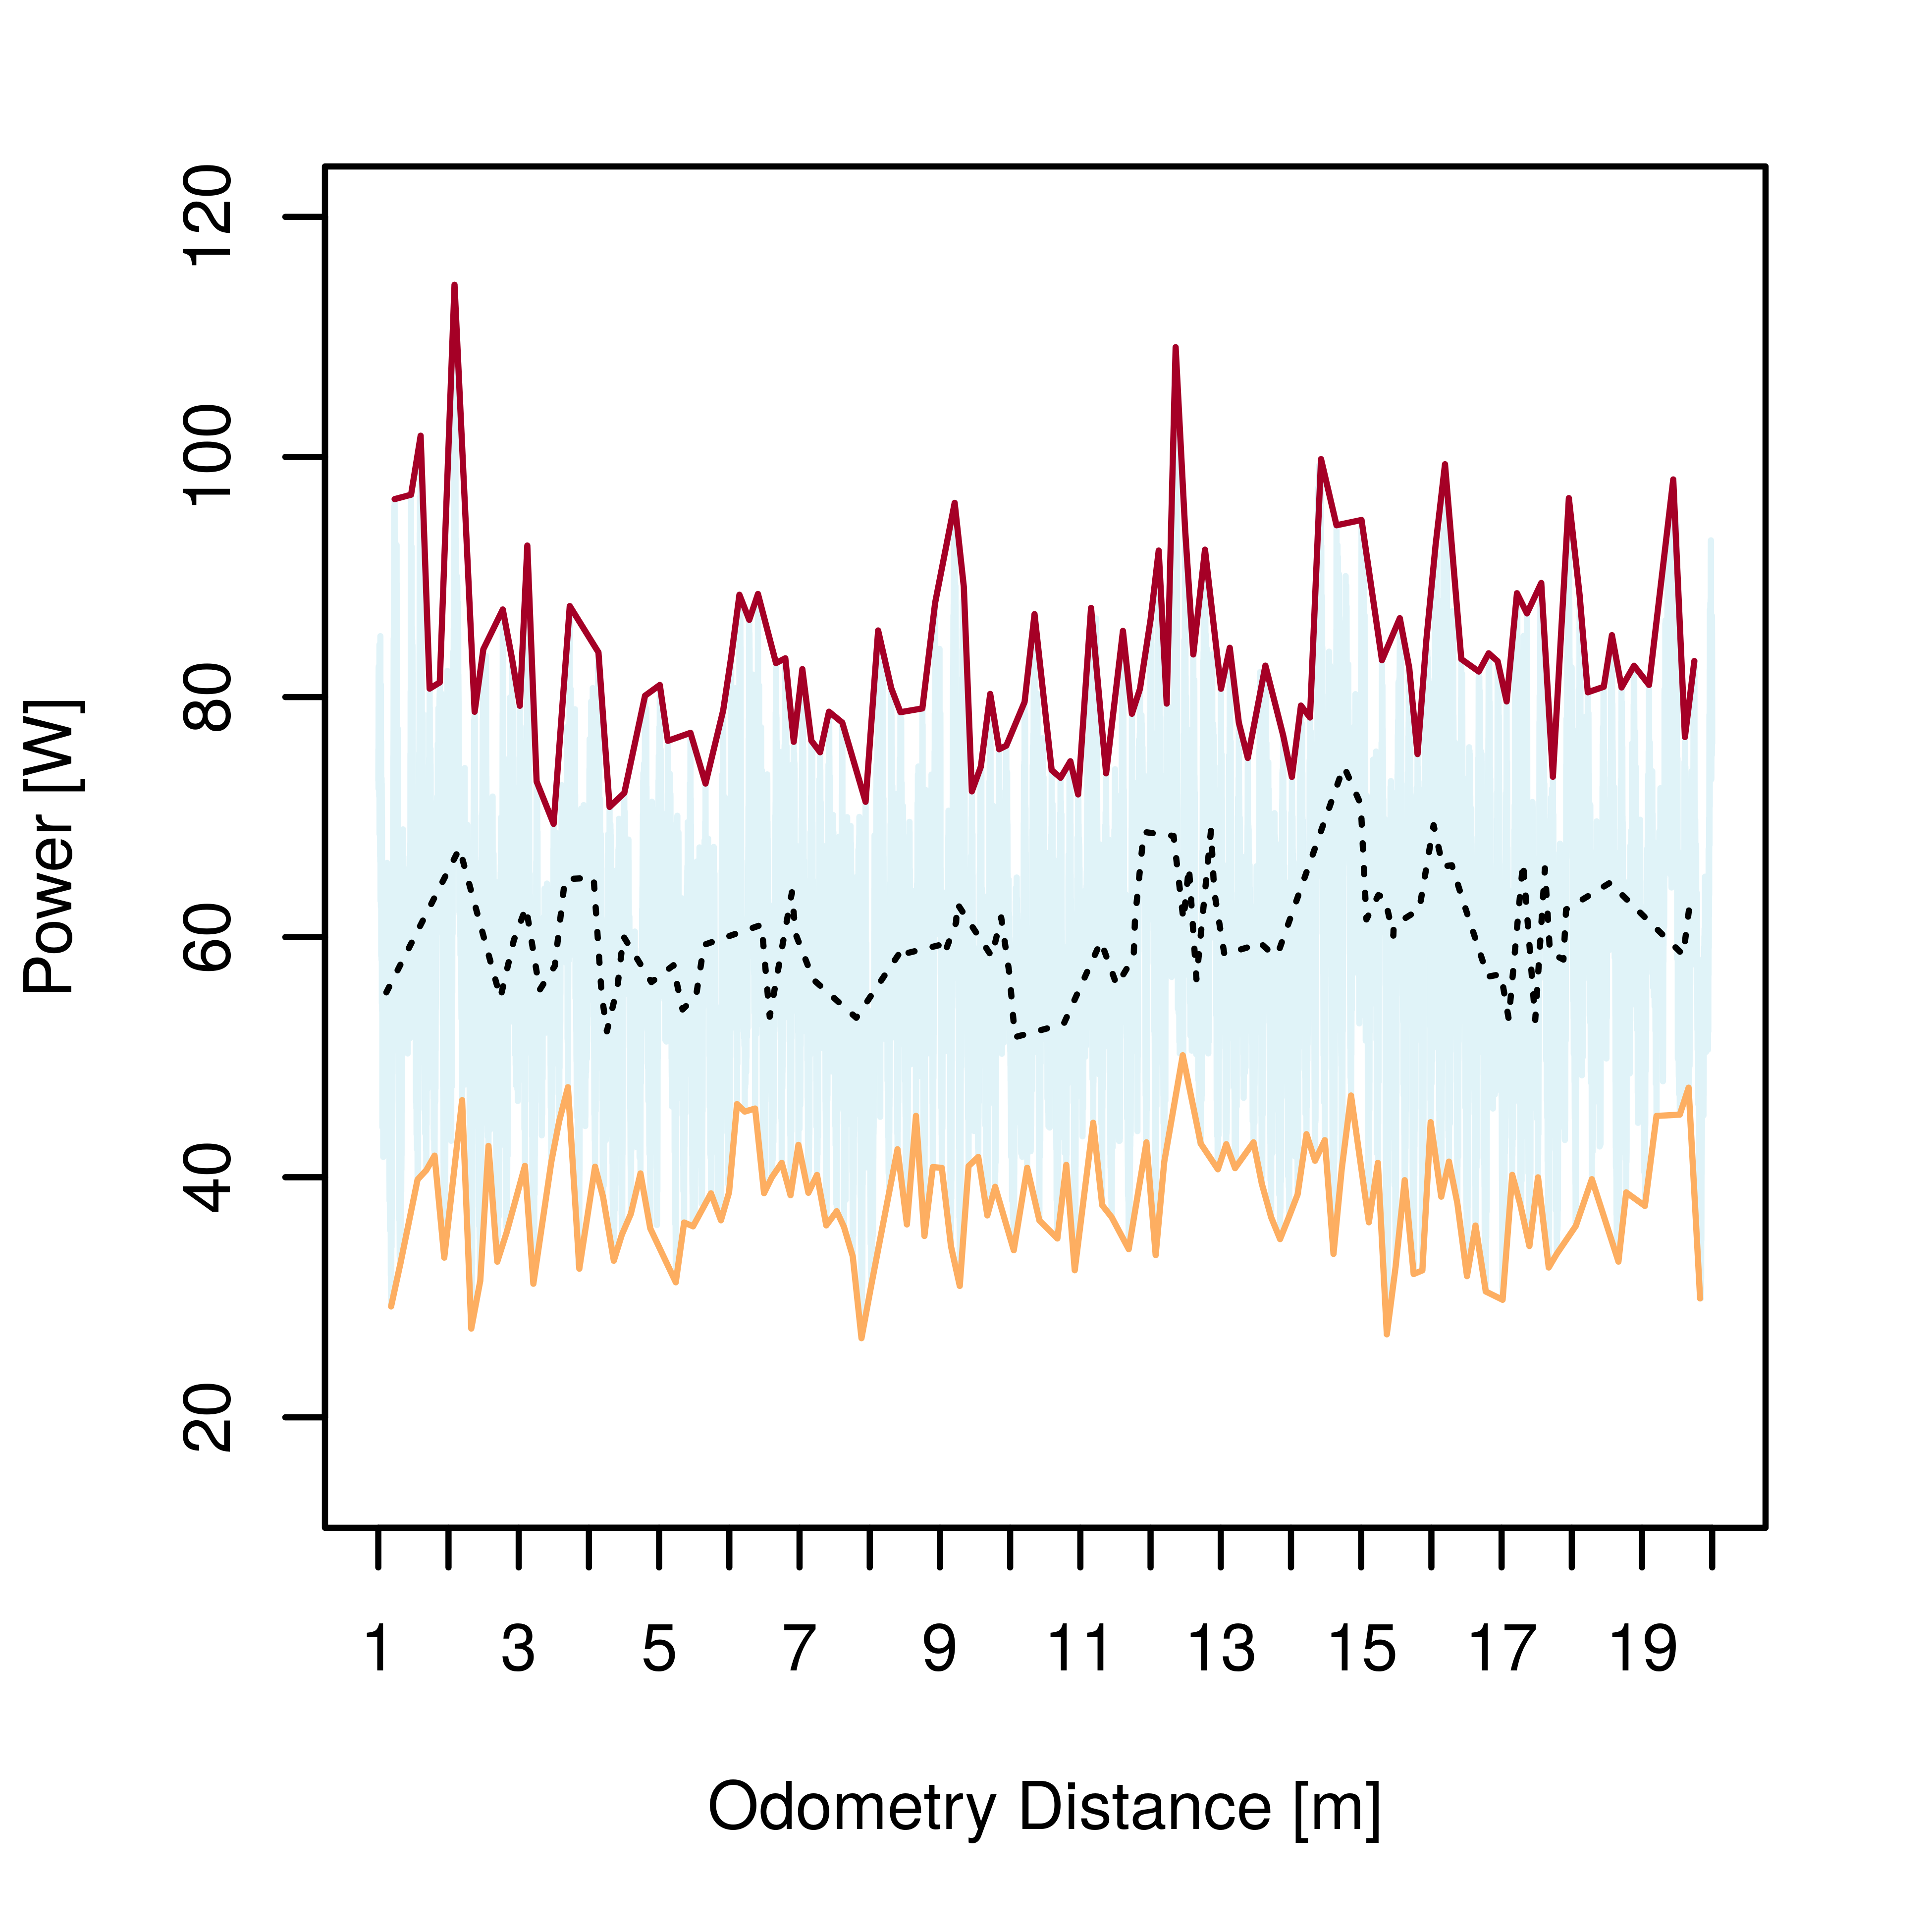
\includegraphics[height=\graphicsHeight]{sections/design/power-budget/plots/locomotion-power-draw-on-flat-terrain-1.png}
        \subcaption{Run \#1}
        \label{fig:plot:sub:sherpatt-flat-terrain-power-draw-1}
    \end{subfigure}\hfill
    \begin{subfigure}[t]{\subfigureWidth}
        \centering
        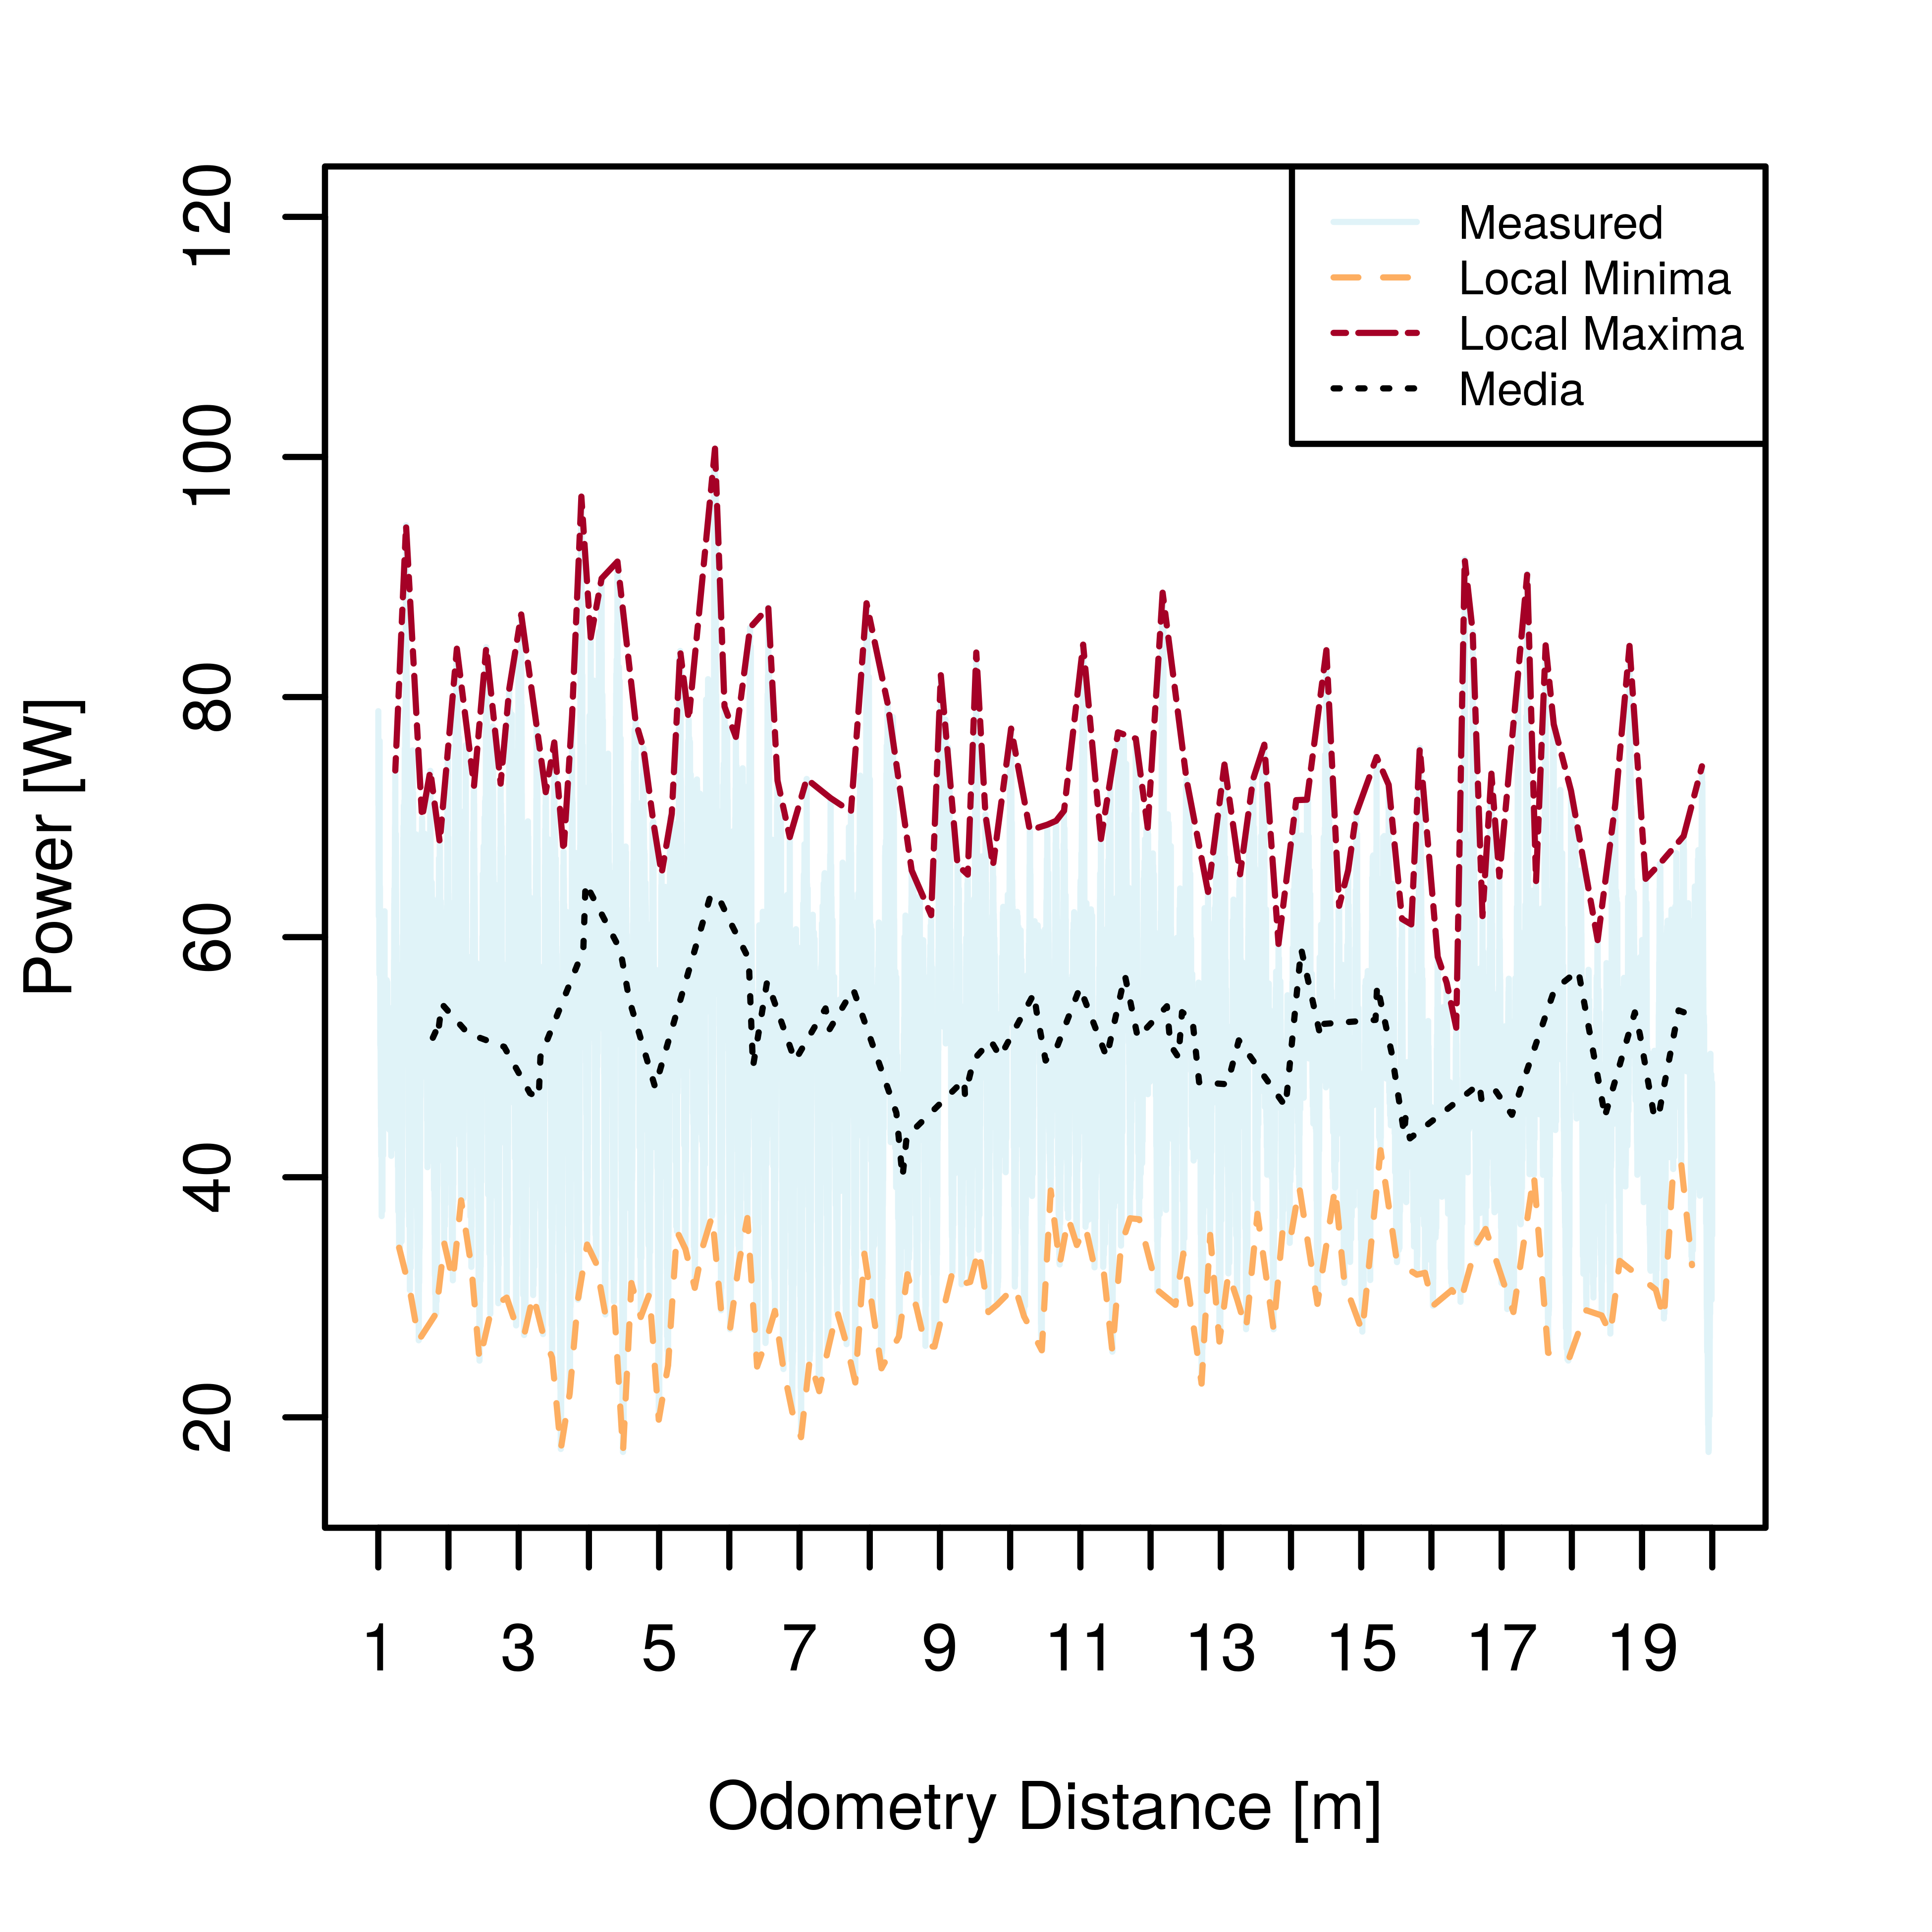
\includegraphics[height=\graphicsHeight]{sections/design/power-budget/plots/locomotion-power-draw-on-flat-terrain-2.png}
  		\subcaption{Run \#2}
		\label{fig:plot:sub:sherpatt-flat-terrain-power-draw-2}
	\end{subfigure}\\[0.8ex]
    \caption[Propulsion power draw for a flat terrain traverse during SherpaTT Mars analogue field tests in Utah]
            {Propulsion power draw for a flat terrain traverse during SherpaTT Mars analogue field tests in Utah.}
    \label{fig:plot:sherpatt-flat-terrain-power-draw}
\vspace{-2ex}
\end{figure}

Measurements are summarised in \refTab{tab:sherpatt-flat-terrain-global-minimum-maximum-and-medium-power-draws}. To eliminate power draw fluctuations from the analysis, only local media values were considered. Local media were selected rather than the worst-case local maxima on the basis of the assumptions made in \refSec{sec:PowerBudget:PropulsionPowerBudget}. For flat terrain traverses, a worst-case maximum power draw of \SI{74}{\watt} is observed in close accordance with the initial estimate obtained from \refEqn{eq:InitialPropulsionPowerEstimate}.

\begin{table}[h]
\footnotesize
\centering
\caption[Global minimum, maximum, and medium of traced local minima, maxima, and media for SherpaTT flat terrain propulsion power draw lines]
    {Global minimum, maximum, and medium of traced local minima, maxima, and media for SherpaTT flat terrain propulsion power draw lines.}
\label{tab:sherpatt-flat-terrain-global-minimum-maximum-and-medium-power-draws}
\begin{tabular}{llccc}
\cline{3-5}
\multicolumn{2}{l|}{\multirow{2}{*}{}} & \multicolumn{3}{c|}{\textbf{Power Draw {[}W{]}}} \\ \cline{3-5}
\multicolumn{2}{l|}{} & \multicolumn{1}{c|}{\textbf{\begin{tabular}[c]{@{}c@{}}Global Minimum\end{tabular}}} & \multicolumn{1}{c|}{\textbf{\begin{tabular}[c]{@{}c@{}}Global Maximum\end{tabular}}} & \multicolumn{1}{c|}{\textbf{\begin{tabular}[c]{@{}c@{}}Global Media\end{tabular}}} \\ \hline
\multicolumn{1}{|c|}{\multirow{4}{*}{\textbf{Run \#1}}} & \multicolumn{1}{l|}{\textbf{Measured}} & \multicolumn{1}{c|}{27} & \multicolumn{1}{c|}{114} & \multicolumn{1}{c|}{60} \\ \cline{2-5}
\multicolumn{1}{|c|}{} & \multicolumn{1}{l|}{\textbf{Local Minima}} & \multicolumn{1}{c|}{27} & \multicolumn{1}{c|}{50} & \multicolumn{1}{c|}{38} \\ \cline{2-5}
\multicolumn{1}{|c|}{} & \multicolumn{1}{l|}{\textbf{Local Maxima}} & \multicolumn{1}{c|}{69} & \multicolumn{1}{c|}{114} & \multicolumn{1}{c|}{83} \\ \cline{2-5}
\multicolumn{1}{|c|}{} & \multicolumn{1}{l|}{\textbf{Local Media}} & \multicolumn{1}{c|}{52} & \multicolumn{1}{c|}{74} & \multicolumn{1}{c|}{61} \\ \hhline{|=|=|=|=|=|}
\multicolumn{1}{|l|}{\multirow{4}{*}{\textbf{Run \#2}}} & \multicolumn{1}{l|}{\textbf{Measured}} & \multicolumn{1}{c|}{17} & \multicolumn{1}{c|}{101} & \multicolumn{1}{c|}{51} \\ \cline{2-5}
\multicolumn{1}{|l|}{} & \multicolumn{1}{l|}{\textbf{Local Minima}} & \multicolumn{1}{c|}{17} & \multicolumn{1}{c|}{42} & \multicolumn{1}{c|}{30} \\ \cline{2-5}
\multicolumn{1}{|l|}{} & \multicolumn{1}{l|}{\textbf{Local Maxima}} & \multicolumn{1}{c|}{52} & \multicolumn{1}{c|}{101} & \multicolumn{1}{c|}{74} \\ \cline{2-5}
\multicolumn{1}{|l|}{} & \multicolumn{1}{l|}{\textbf{Local Media}} & \multicolumn{1}{c|}{40} & \multicolumn{1}{c|}{64} & \multicolumn{1}{c|}{52} \\ \hline
 &  & \multicolumn{1}{l}{} & \multicolumn{1}{l}{} & \multicolumn{1}{l}{} \\
 &  & \multicolumn{1}{l}{} & \multicolumn{1}{l}{} & \multicolumn{1}{l}{}
\end{tabular}
\end{table}


\subsubsection{Upslope Terrain Traverse}
\label{sec:PowerBudget:PropulsionPowerBudget:UpslopeTerrainTraverse}
Propulsion power draws on a steep uplsope were measured along an approximately \SI{16}{\meter} track and are shown in \refFig{fig:plot:sub:sherpatt-disaggregated-upslope-terrain-power-draw-locomotion}. An initial estimate of \SI{132}{\watt} is obtained using \refEqn{eq:InitialPropulsionPowerEstimate}. A worst case \SI{98}{\percent} suspension system's share of the total propulsion power is taken from \citeother{Cordes2018} for data collected from a steep slope outdoor setting. The drive and suspension power draw components are shown in \refFig{fig:plot:sub:sherpatt-disaggregated-upslope-terrain-power-draw-drive} and \refFig{fig:plot:sub:sherpatt-disaggregated-upslope-terrain-power-draw-suspension}, respectively.

\begin{figure}[h]
\captionsetup[subfigure]{justification=centering}
\vspace{-2ex}
	\centering
    %% setup sizes
    \setlength{\subfigureWidth}{0.32\textwidth}
    \setlength{\graphicsHeight}{50mm}
    %% kill hyper-link highlighting
    \hypersetup{hidelinks=true}%
    %% the figures
	\begin{subfigure}[t]{\subfigureWidth}
        \centering
        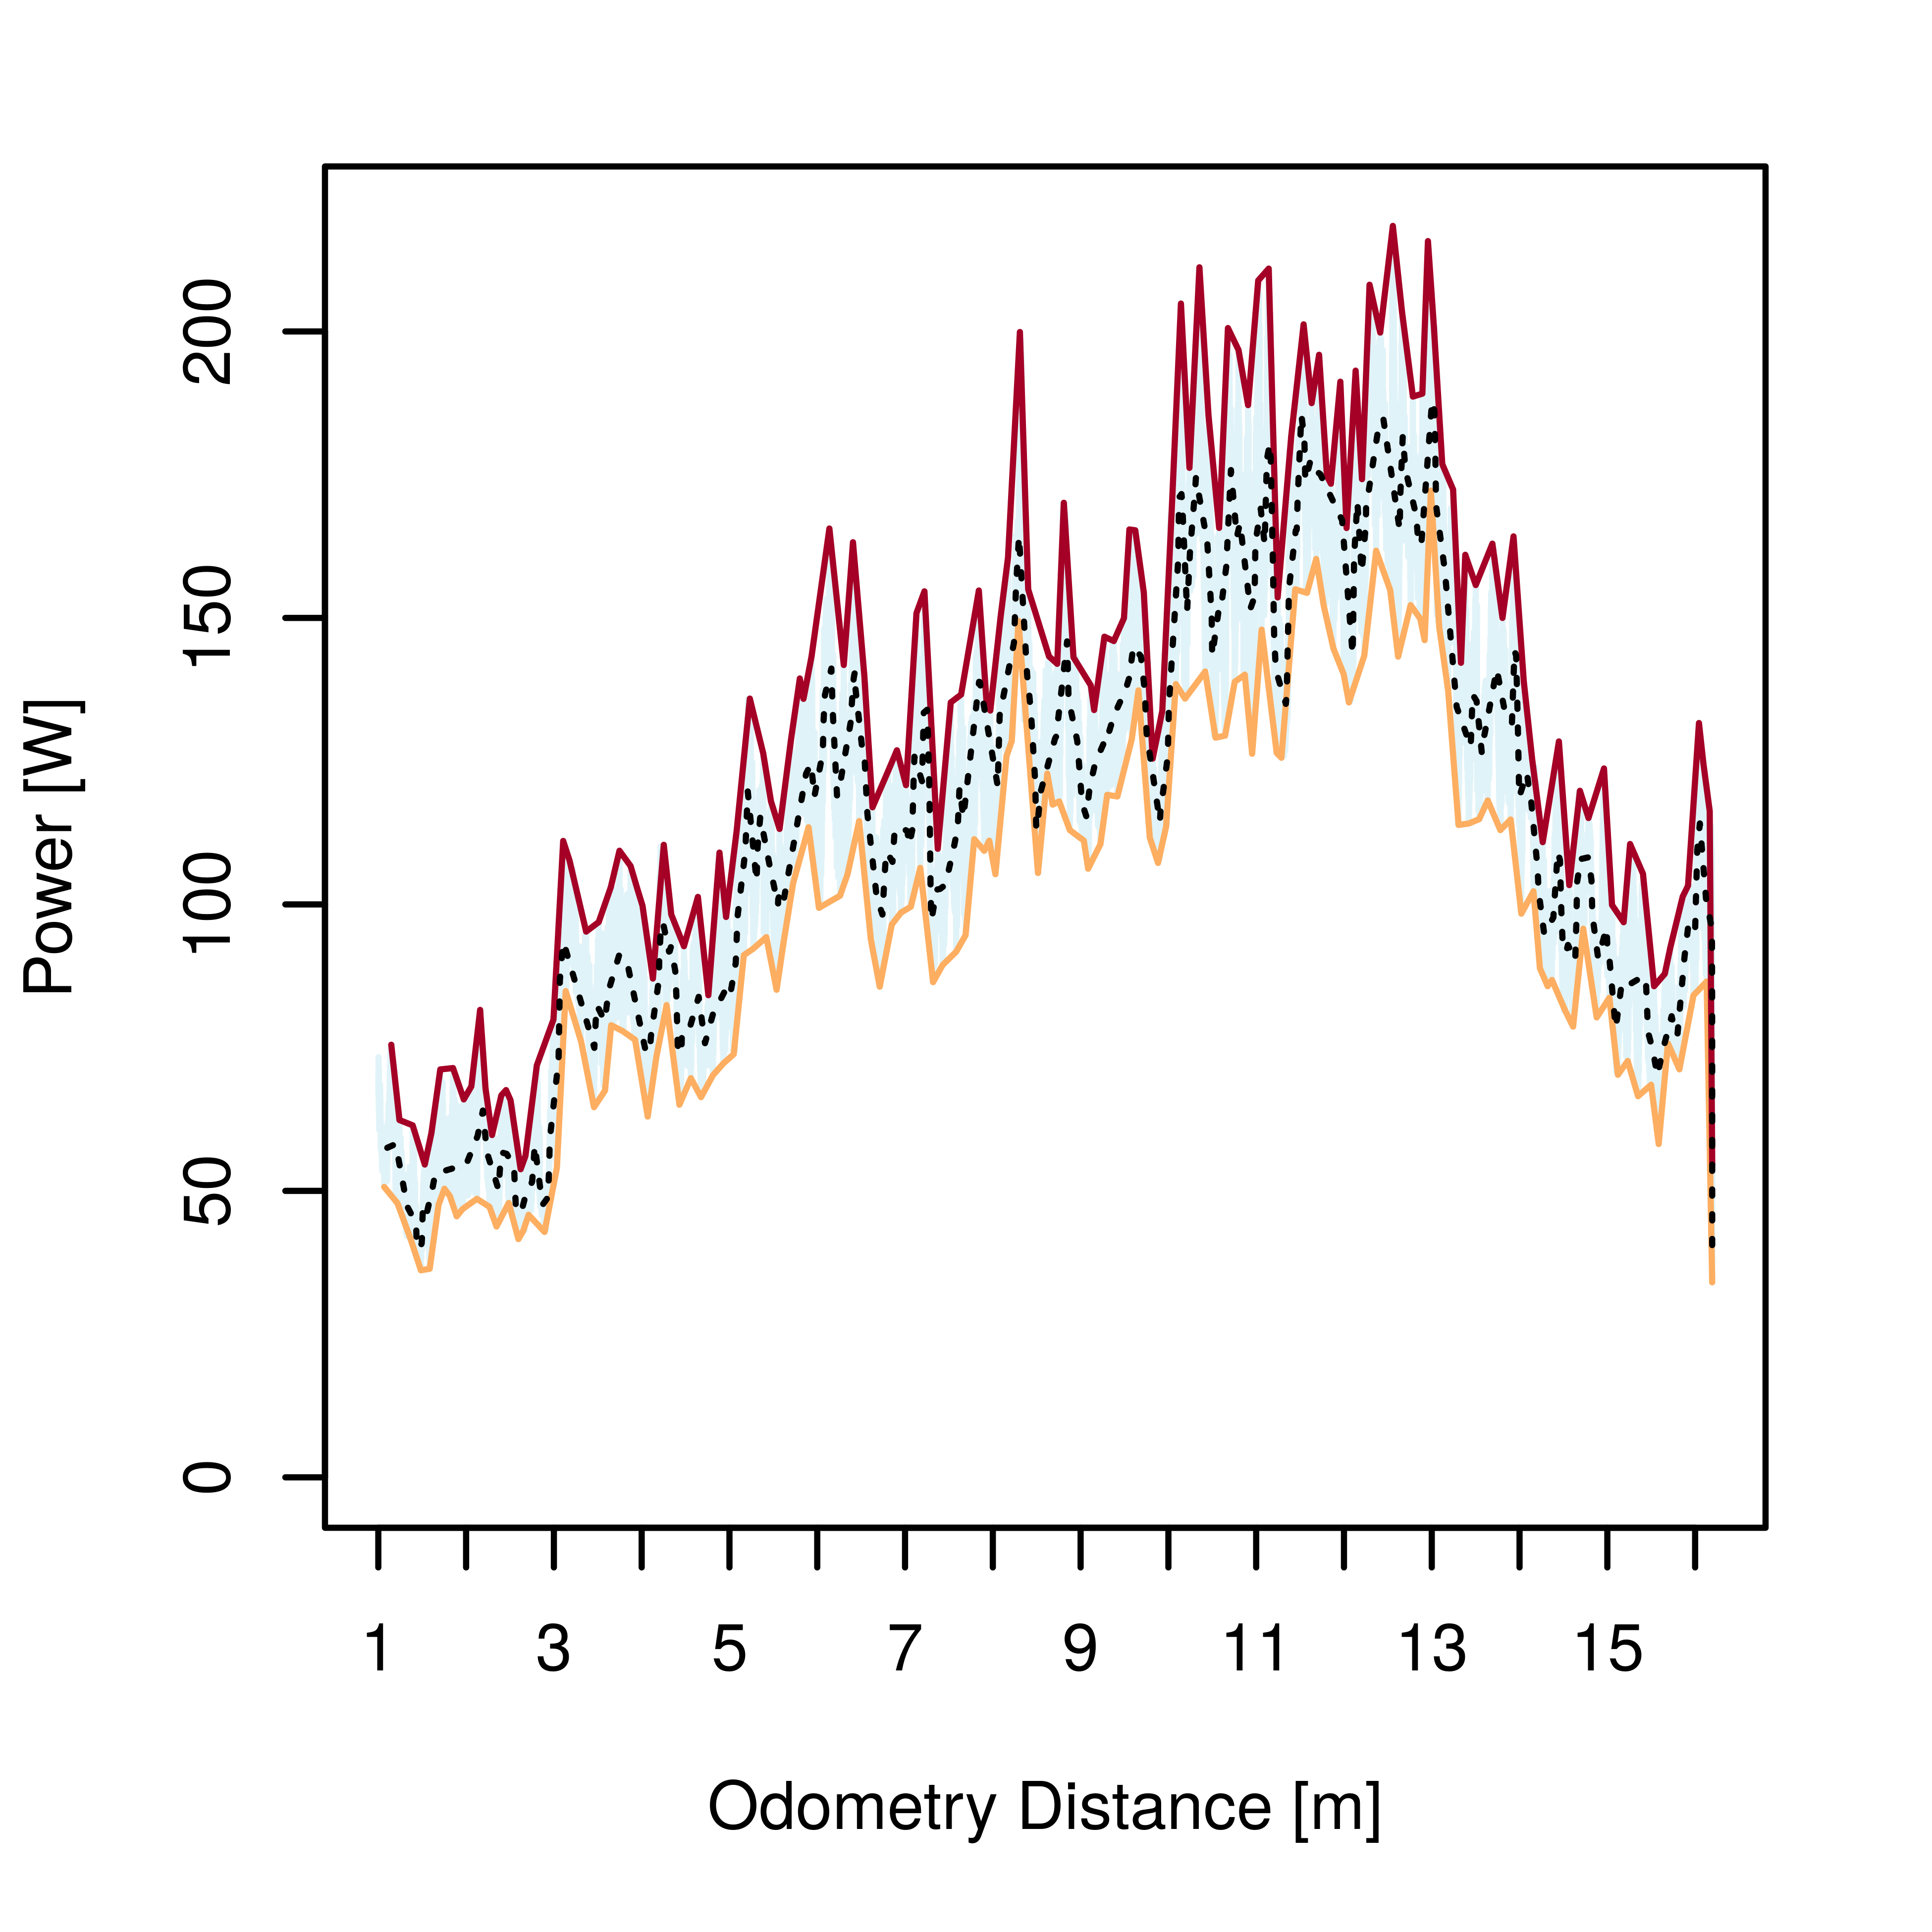
\includegraphics[height=\graphicsHeight]{sections/design/power-budget/plots/locomotion-power-draw-on-upslope-terrain.png}
  		\subcaption{Propulsion}
		\label{fig:plot:sub:sherpatt-disaggregated-upslope-terrain-power-draw-locomotion}
	\end{subfigure}\hfill
	\begin{subfigure}[t]{\subfigureWidth}
        \centering
        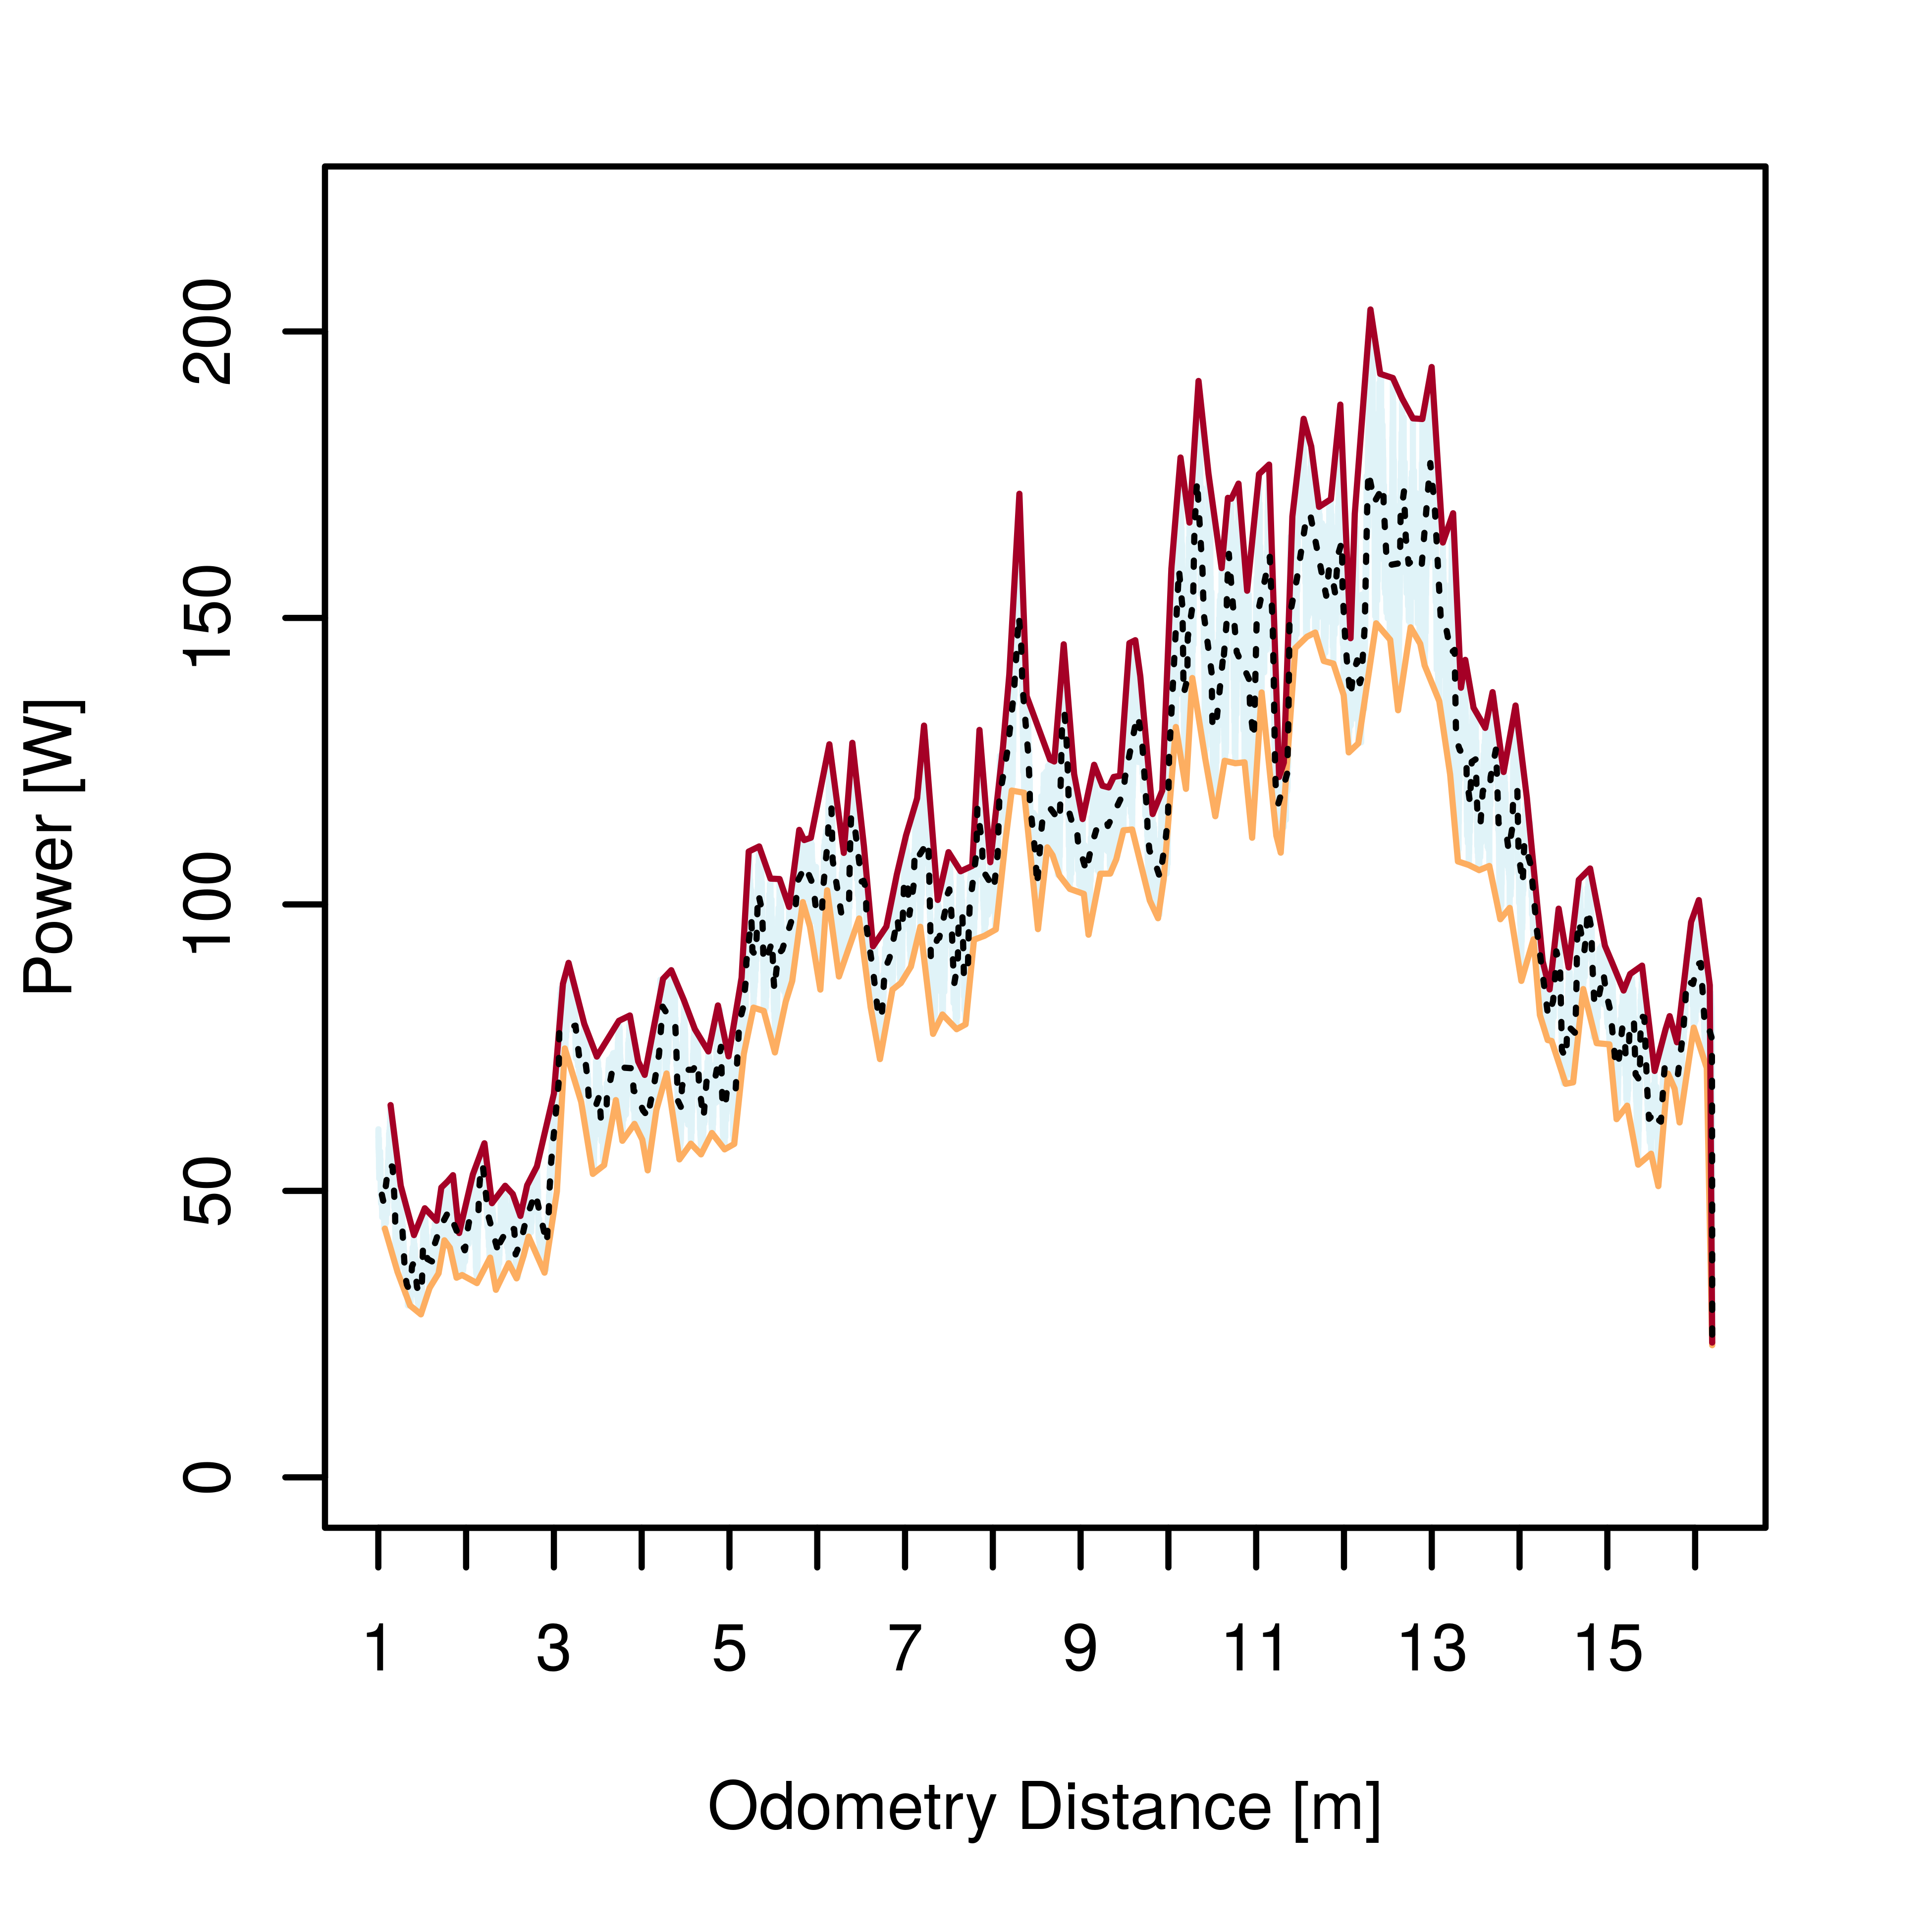
\includegraphics[height=\graphicsHeight]{sections/design/power-budget/plots/drive-power-draw-on-upslope-terrain.png}
  		\subcaption{Drive}
		\label{fig:plot:sub:sherpatt-disaggregated-upslope-terrain-power-draw-drive}
	\end{subfigure}\hfill
    \begin{subfigure}[t]{\subfigureWidth}
        \centering
        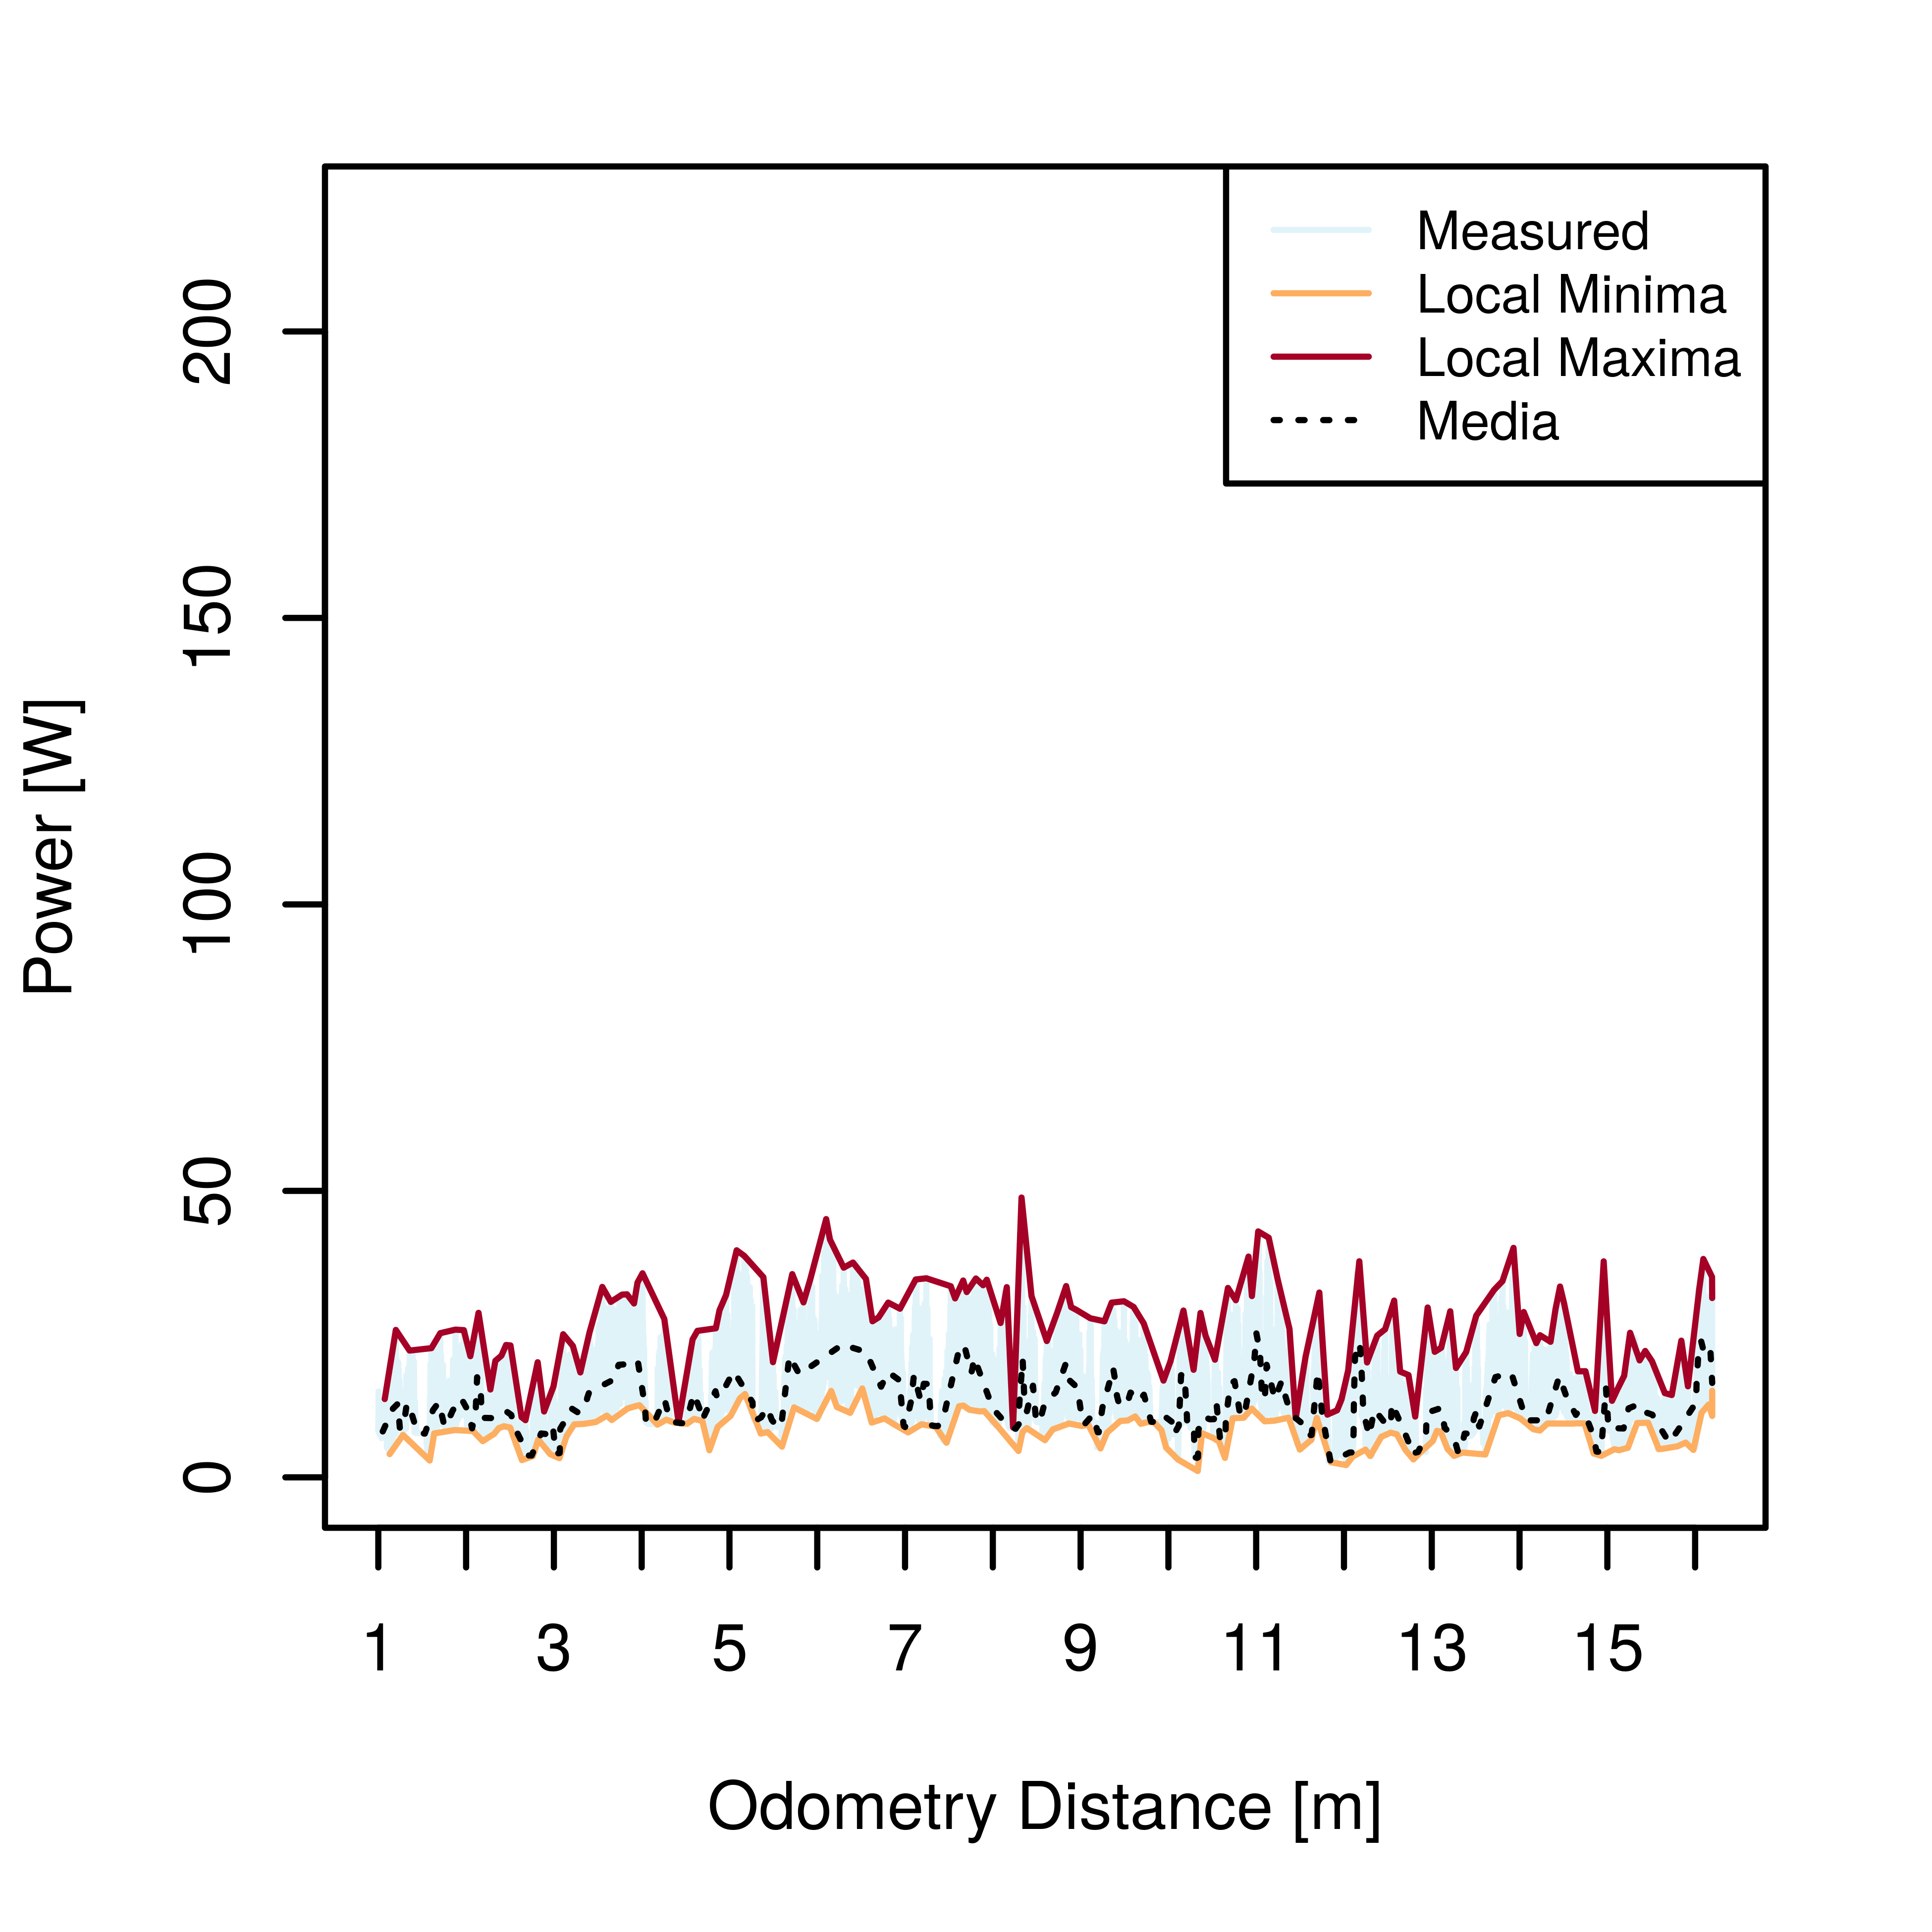
\includegraphics[height=\graphicsHeight]{sections/design/power-budget/plots/suspension-power-draw-on-upslope-terrain.png}
  		\subcaption{Suspension}
		\label{fig:plot:sub:sherpatt-disaggregated-upslope-terrain-power-draw-suspension}
	\end{subfigure}\\[0.8ex]
    \caption[Disaggregated measurements of power draw for upslope terrain traverse during SherpaTT Mars analogue field tests in Utah]
            {Disaggregated measurements of power draw for upslope terrain traverse during SherpaTT Mars analogue field tests in Utah: (a) = (b) + (c).}
    \label{fig:plot:sherpatt-disaggregated-upslope-terrain-power-draw}
\vspace{-2ex}
\end{figure}

An uplsope traverse has no discernable effect on the suspension power draw, however; there is a clear gradual increase in the drive power draw. The global maximum, minimum, and medium of the traced local minima, maxima, and media power draw lines are presented in \refTab{tab:sherpatt-upslope-terrain-global-minimum-maximum-and-medium-power-draws}.

\begin{table}[h]
\footnotesize
\centering
\caption[Global minimum, maximum, and medium of traced local minima, maxima, and media for SherpaTT upslope terrain traverse propulsion power draw lines]
    {Global minimum, maximum, and medium of traced local minima, maxima, and media for SherpaTT upslope terrain traverse propulsion power draw lines.}
\label{tab:sherpatt-upslope-terrain-global-minimum-maximum-and-medium-power-draws}
\begin{tabular}{l|c|c|c|}
\cline{2-4}
\multicolumn{1}{c|}{\multirow{2}{*}{\textbf{}}} & \multicolumn{3}{c|}{\textbf{Power Draw {[}W{]}}} \\ \cline{2-4}
\multicolumn{1}{c|}{} & \textbf{\begin{tabular}[c]{@{}c@{}}Global Minimum\end{tabular}} & \textbf{\begin{tabular}[c]{@{}c@{}}Global Maximum\end{tabular}} & \textbf{\begin{tabular}[c]{@{}c@{}}Global Media\end{tabular}} \\ \hline
\multicolumn{1}{|l|}{\textbf{Measured}} & 34 & 218 & 114 \\ \hline
\multicolumn{1}{|l|}{\textbf{Local Minima}} & 34 & 172 & 98 \\ \hline
\multicolumn{1}{|l|}{\textbf{Local Maxima}} & 54 & 218 & 133 \\ \hline
\multicolumn{1}{|l|}{\textbf{Local Media}} & 40 & 188 & 18 \\ \hline
\end{tabular}
\end{table}


\refFig{fig:plot:sherpatt-upslope-terrain-power-draw} overlaps the propulsion local media power draws with the tackled slope angles. The steepest slope angle is \SI{28}{\degree} for an average of \SI{17.52}{\degree}. Slope angle increases are consistently followed by power draw spikes, i.e. at approximately 3, 4, 5, 6, 8, and 9 \si{\meter} in the odometry measurements. Inversely, slope angle decreases are followed by power draws troughs at approximately 11, 13, 14, and 16 \si{\meter}. Slope angles are measured in \SI{1}{meter} discret intervals.

\begin{figure}[h]
  \centering
  \hypersetup{linkcolor=captionTextColor}
  \includegraphics[width=0.8\linewidth]{sections/design/power-budget/plots/minima-locomotion-power-draws-on-upslope-terrain.png}\\
  \caption[Mean Propulsion power draw for an upslope terrain traverse during SherpaTT Utah field test campaign.]
          {Mean Propulsion power draw for an upslope terrain traverse during SherpaTT Utah field test campaign.}
  \label{fig:plot:sherpatt-upslope-terrain-power-draw}
\end{figure}


The power draws trough following the slope angle change from \SI{28}{\degree} to \SI{20}{\degree} at the \SI{11}{\meter} mark is subsequently followed by an unusual power draw increase and fluctuation. These measurements are discarded as outliers. \refTab{tab:sherpatt-upslope-terrain-local-media-measurement-summary} summarises the minimum, maximum, and mean local media propulsion power draws that are measured for different slope angles. Discarding the outlier measurements subsequent to the slope angle change from \SI{28}{\degree} to \SI{20}{\degree} at the \SI{11}{\meter} to \SI{13}{\meter} portion of the track, the maximum mean local media propulsion power draw is \SI{146}{\watt}. This is close agreement with the initial estimate of \SI{132}{\watt} obtained with \refEqn{eq:InitialPropulsionPowerEstimate}.

\begin{table}[h]
\footnotesize
\centering
\caption[SherpaTT mean propulsion power draw measurements for different slope sections]
    {SherpaTT mean propulsion power draw measurements for different slope sections.}
\label{tab:sherpatt-upslope-terrain-local-media-measurement-summary}
\begin{tabular}{cc|c|c|c|}
\cline{3-5}
\multicolumn{1}{l}{} & \multicolumn{1}{l|}{} & \multicolumn{3}{c|}{\textbf{Power {[}W{]}}} \\ \hline
\multicolumn{1}{|l|}{\textbf{Distance {[}m{]}}} & \multicolumn{1}{l|}{\textbf{Slope Angle {[}deg{]}}} & \multicolumn{1}{l|}{\textbf{Minimum}} & \multicolumn{1}{l|}{\textbf{Maximum}} & \multicolumn{1}{l|}{\textbf{Mean}} \\ \hline
\multicolumn{1}{|c|}{\textbf{1 $<$ x $\leq$ 3}} & 10 & 40 & 64 & 51 \\ \hline
\multicolumn{1}{|c|}{\textbf{3 $<$ x $\leq$ 4}} & 11 & 73 & 93 & 85 \\ \hline
\multicolumn{1}{|c|}{\textbf{4 $<$ x $\leq$ 5}} & 15 & 74 & 87 & 83 \\ \hline
\multicolumn{1}{|c|}{\textbf{5 $<$ x $\leq$ 6}} & 16 & 85 & 125 & 107 \\ \hline
\multicolumn{1}{|c|}{\textbf{6 $<$ x $\leq$ 7}} & 28 & 98 & 141 & 123 \\ \hline
\multicolumn{1}{|c|}{\textbf{7 $<$ x $\leq$ 8}} & 22 & 97 & 139 & 116 \\ \hline
\multicolumn{1}{|c|}{\textbf{8 $<$ x $\leq$ 9}} & 25 & 113 & 164 & 133 \\ \hline
\multicolumn{1}{|c|}{\textbf{9 $<$ x $\leq$ 11}} & 28 & 114 & 176 & 146 \\ \hline
\multicolumn{1}{|c|}{\textbf{11 $<$ x $\leq$ 13}} & 20 & 135 & 188 & 167 \\ \hline
\multicolumn{1}{|c|}{\textbf{13 $<$ x $\leq$ 14}} & 15 & 119 & 123 & 145 \\ \hline
\multicolumn{1}{|c|}{\textbf{14 $<$ x $\leq$ 16}} & 10 & 70 & 186 & 94 \\ \hline
\end{tabular}
\end{table}


\subsection{Traverse Power Budget}
\label{sec:PowerBudget:PowerBudget:TraversePowerBudget}
A worst case daily insolation for an optical depth of $\tau = 1$ is used to determine the energy requirements of the flat and upslope traverse reference Sols. These are taken from \refTab{tab:insolation-iani-chaos-clear-and-dusty-days} for Iani Chaos and \refTab{tab:insolation-ismenius-cavus-clear-and-dusty-days} for Ismenius Cavus. The minimum required traverse distance is assumed to be \SI{5}{\meter} at both mission sites.

\subsubsection{Flat Traverse}
\label{sec:Design:PowerBudget:TraversePowerBudget:FlatTraverse}

Power and duration of \textit{DTE Communication}, \textit{Science Stop - Short}, and \textit{Hibernation} modes are taken from \citeother{CDF2014} and assigned to the reference Sols presented in Section \ref{sec:ReferenceSols:ReferenceSols}. Power draw estimates made in \refSec{sec:PowerBudget:PropulsionPowerBudget:FlatTerrainTraverse} and \refSec{sec:PowerBudget:PropulsionPowerBudget:UpslopeTerrainTraverse} are used for \textit{Traverse} modes. Power draw for the \textit{Optimal Pose} mode is equated to that of the rover's flat terrain propulsion power. This mode is estimated to require up to \SI{10}{\minute} to complete. The worst case power budget for the reference \textit{Flat Traverse Sol} is shown in \refTab{tab:worst-case-traverse-sol-power-budget}.

\begin{table}[h]
\footnotesize
\centering
\caption[Worst-case mission site flat terrain traverse Sol power budget]
    {Worst-case mission site flat terrain traverse Sol power budget for $\tau=1$.}
\label{tab:worst-case-traverse-sol-power-budget}
\begin{tabular}{lc|c|c|c|c|}
\cline{3-6}
 & \textbf{} & \multicolumn{2}{c|}{\textbf{\begin{tabular}[c]{@{}c@{}}Iani Chaos\\ $Ls=\SI{81}{\degree}$\end{tabular}}} & \multicolumn{2}{c|}{\textbf{\begin{tabular}[c]{@{}c@{}}Ismenius Cavus\\ $Ls=\SI{273}{\degree}$\end{tabular}}} \\ \hline
\multicolumn{1}{|l|}{\textbf{Mode}} & \textbf{P {[}W{]}} & \textbf{t {[}min{]}} & \textbf{E {[}Wh{]}} & \textbf{t {[}min{]}} & \textbf{E {[}Wh{]}} \\ \hline
\multicolumn{1}{|l|}{\textbf{Idle - Day}} & 29 & 603 & 291 & 464 & 224 \\ \hline
\multicolumn{1}{|l|}{\textbf{DTE Communication}} & 52 & 35 & 30 & 35 & 30 \\ \hline
\multicolumn{1}{|l|}{\textbf{Traverse - Flat}} & 113\footnote{Power draws taken from \citeother{CDF2014} for Communications, \ac{DHS}, \ac{GNC}, and \ac{PCDU} are added to the \SI{75}{\watt} flat terrain propulsion power draw resulting in a total \textit{Traverse Mode} power budget of \SI{113}{\watt}.} & 4.8 & 9 & 4.8 & 9 \\ \hline
\multicolumn{1}{|l|}{\textbf{Science Stop - Short}} & 60 & 60 & 60 & 60 & 60 \\ \hline
\multicolumn{1}{|l|}{\textbf{Optimal Pose}} & 75 & 12 & 13 & 10 & 13 \\ \hline
\multicolumn{1}{|l|}{\textbf{Idle - Night}} & 20 & 242 & 242 & 866 & 289 \\ \hline
\multicolumn{1}{|r|}{\textbf{Total}} & \textbf{349} & \textbf{1440} & \textbf{646} & \textbf{1440} & \textbf{625} \\ \hline
\multicolumn{1}{|r|}{\textbf{Total +20\% System Margin}} & \textbf{419} & - & \textbf{775} & - & \textbf{750} \\ \hline
\end{tabular}
\end{table}


The total energy requirements for these worst case reference Sols are used as the minimum energy output when sizing the \ac{SA}. A \SI{20}{\percent} system margin is applied to account for inefficiencies such as \ac{PCDU} losses.

\subsubsection{Upslope Traverse}
\label{sec:Design:PowerBudget:TraversePowerBudget:UpslopeTraverse}
The worst case upslope traverse reference Sols shown in \refTab{tab:worst-case-upslope-traverse-sol-power-budget} only differ from their flat traverse equivalents by the \textit{Traverse mode} power draw. It is increased from \SI{75}{\watt} to \SI{150}{\watt}.

\begin{table}[h]
\footnotesize
\centering
\caption[Worst-case upslope traverse Sol power budget at mission sites]
    {Worst-case upslope traverse Sol power budget at mission sites for $\tau =1$.}
\label{tab:worst-case-upslope-traverse-sol-power-budget}
\begin{tabular}{lc|c|c|c|c|}
\cline{3-6}
 & \textbf{} & \multicolumn{2}{c|}{\textbf{\begin{tabular}[c]{@{}c@{}}Iani Chaos\\ $Ls=\SI{81}{\degree}$\end{tabular}}} & \multicolumn{2}{c|}{\textbf{\begin{tabular}[c]{@{}c@{}}Ismenius Cavus\\ $Ls=\SI{273}{\degree}$\end{tabular}}} \\ \hline
\multicolumn{1}{|l|}{\textbf{Mode}} & \textbf{P {[}W{]}} & \textbf{t {[}min{]}} & \textbf{E {[}Wh{]}} & \textbf{t {[}min{]}} & \textbf{E {[}Wh{]}} \\ \hline
\multicolumn{1}{|l|}{\textbf{Idle - Day}} & 29 & 603 & 291 & 464 & 224 \\ \hline
\multicolumn{1}{|l|}{\textbf{DTE Communication}} & 52 & 35 & 30 & 35 & 30 \\ \hline
\multicolumn{1}{|l|}{\textbf{Traverse - Upslope}} & 188\footnote{Power draws taken from \citeother{CDF2014} for Communications, \ac{DHS}, \ac{GNC}, and \ac{PCDU} are added to the \SI{150}{\watt} flat terrain propulsion power draw resulting in a total \textit{Traverse Mode} power budget of \SI{188}{\watt}.} & 4.8 & 9 & 4.8 & 15 \\ \hline
\multicolumn{1}{|l|}{\textbf{Science Stop - Short}} & 60 & 60 & 60 & 60 & 60 \\ \hline
\multicolumn{1}{|l|}{\textbf{Optimal Pose}} & 75 & 12 & 13 & 10 & 13 \\ \hline
\multicolumn{1}{|l|}{\textbf{Idle - Night}} & 20 & 242 & 242 & 866 & 289 \\ \hline
\multicolumn{1}{|r|}{\textbf{Total}} & \textbf{424} & \textbf{1440} & \textbf{652} & \textbf{1440} & \textbf{631} \\ \hline
\multicolumn{1}{|r|}{\textbf{Total +20\% System Margin}} & \textbf{509} & - & \textbf{782} & - & \textbf{757} \\ \hline
\end{tabular}
\end{table}


These worst case reference Sols were are considered in \ac{SA} sizing. Regardless, they are presented for the sake of comparative analysis with the flat traverse equivalent.


\subsubsection{Hibernation}
\label{sec:Design:PowerBudget:TraversePowerBudget:Hibernation}
The power budget for the reference \textit{Hibernation Sol} is shown in \refTab{tab:hibernation-sol-power-budget}. The \SI{18}{\watt} power draw is taken from \citeother{CDF2014}.

\begin{table}[h]
\footnotesize
\centering
\caption[Hibernation Sol power budget]
    {Hibernation Sol power budget.}
\label{tab:hibernation-sol-power-budget}
\begin{tabular}{lc|c|c|c|c|}
\cline{3-6}
 & \textbf{} & \multicolumn{2}{c|}{\textbf{Iani Chaos}} & \multicolumn{2}{c|}{\textbf{Ismenius Cavus}} \\ \hline
\multicolumn{1}{|l|}{\textbf{Mode}} & \textbf{P {[}W{]}} & \textbf{t {[}min{]}} & \textbf{E {[}Wh{]}} & \textbf{t {[}min{]}} & \textbf{E {[}Wh{]}} \\ \hline
\multicolumn{1}{|l|}{\textbf{Hibernation - Day}} & 18 & 720 & 216 & 720 & 216 \\ \hline
\multicolumn{1}{|l|}{\textbf{Hibernation - Night}} & 18 & 720 & 216 & 720 & 216 \\ \hline
\multicolumn{1}{|r|}{\textbf{Total}} & \textbf{36} & \textbf{1440} & \textbf{432} & \textbf{1440} & \textbf{432} \\ \hline
\multicolumn{1}{|r|}{\textbf{Total +20\% System Margin}} & \textbf{43} & - & \textbf{518} & - & \textbf{518} \\ \hline
\end{tabular}
\end{table}


\subsection{Summary}
\label{sec:PowerBudget:Summary}
The rover's propulsion power performance was extracted from data collected during the Utah field trials. Reference sols were formalized and a power draw analysis was undertaken in order to determine the rover's worst case energy requirements during traverse and hibernation Sols.
